\documentclass{article}

\usepackage{graphicx}
\usepackage[margin=1.0in]{geometry}
\usepackage{natbib}

\begin{document}



\title{\vspace{-10mm}\bf{\Large{Question 4 of Comp-Astro Midterm}}}
\author{\sc{Jodi Berdis}}
\date{21 Oct 2015}
\maketitle

\vspace{5mm}
\section{Summary of Question 3}

First and foremost, I decided to write my routines in an ipython notebook to save on time and be able to compare my previous notes and homeworks with the work in question 3. In part `a)', I created a function that would compute the value of: $f(x) = x^{3} + x^{2/3}$ as a returned result, with an input parameter of a user-defined `x' variable. In part `b)', I write an integral function to numerically calculate the approximation given on the bottom of the first page of the midterm. This function also required user-input values for the limits of the integral. However, this was only a numerical approximation; in order to correctly solve the integral analytically, for part `c)' and `d)', I wrote a function (that could have been much cleaner with a bit more time) that simulated an "integral-by-hand" approach, emph{i.e.}, taking an indefinite anti-derivative, then plugging in the limits. I'm currently stuck on part `e)'. I have attempted splitting the integral into parts (where the number of parts is defined by the user), and integrating the original function in pieces in order to compute a more accurate result. With a bit more time, I could debug this section of my code, determine at which point I would arrive at 0.1 percent accuracy (where the original integration returned a 0.75 accuracy), and plot these percentages against the user-defined number of pieces into which the integral was split.
\linebreak
\linebreak
Since my code still requires debugging, I have made up values for the result, so that I can at least demonstrate my ability to plot data, as well as insert plots into LaTeX code. The resulting `false' plot is displayed in Figure~\ref{fig:figure_1} below:


\begin{figure}[ht]
\begin{center}
{\sc Figure~\ref{fig:figure_1}}
\linebreak
\linebreak
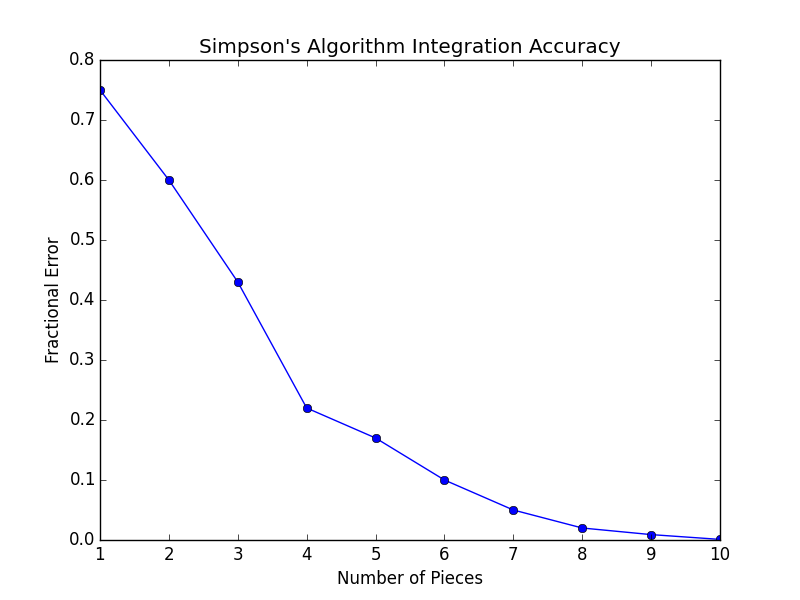
\includegraphics[scale=0.5]{figure_1.png}
\end{center}{
\footnotesize {\sc Figure 1.} Plot depicts the fractional accuracy of the Simpson's Algorithm for Integration.}
\label{fig:figure_1}
\end{figure}



\end{document}
